% ──────────────────────────────────────────────────────────────────────────────
%  Energy Transducer  ·  Figure captions for et_01 – et_06
% ──────────────────────────────────────────────────────────────────────────────

\begin{figure*}[!htbp]
    \centering
    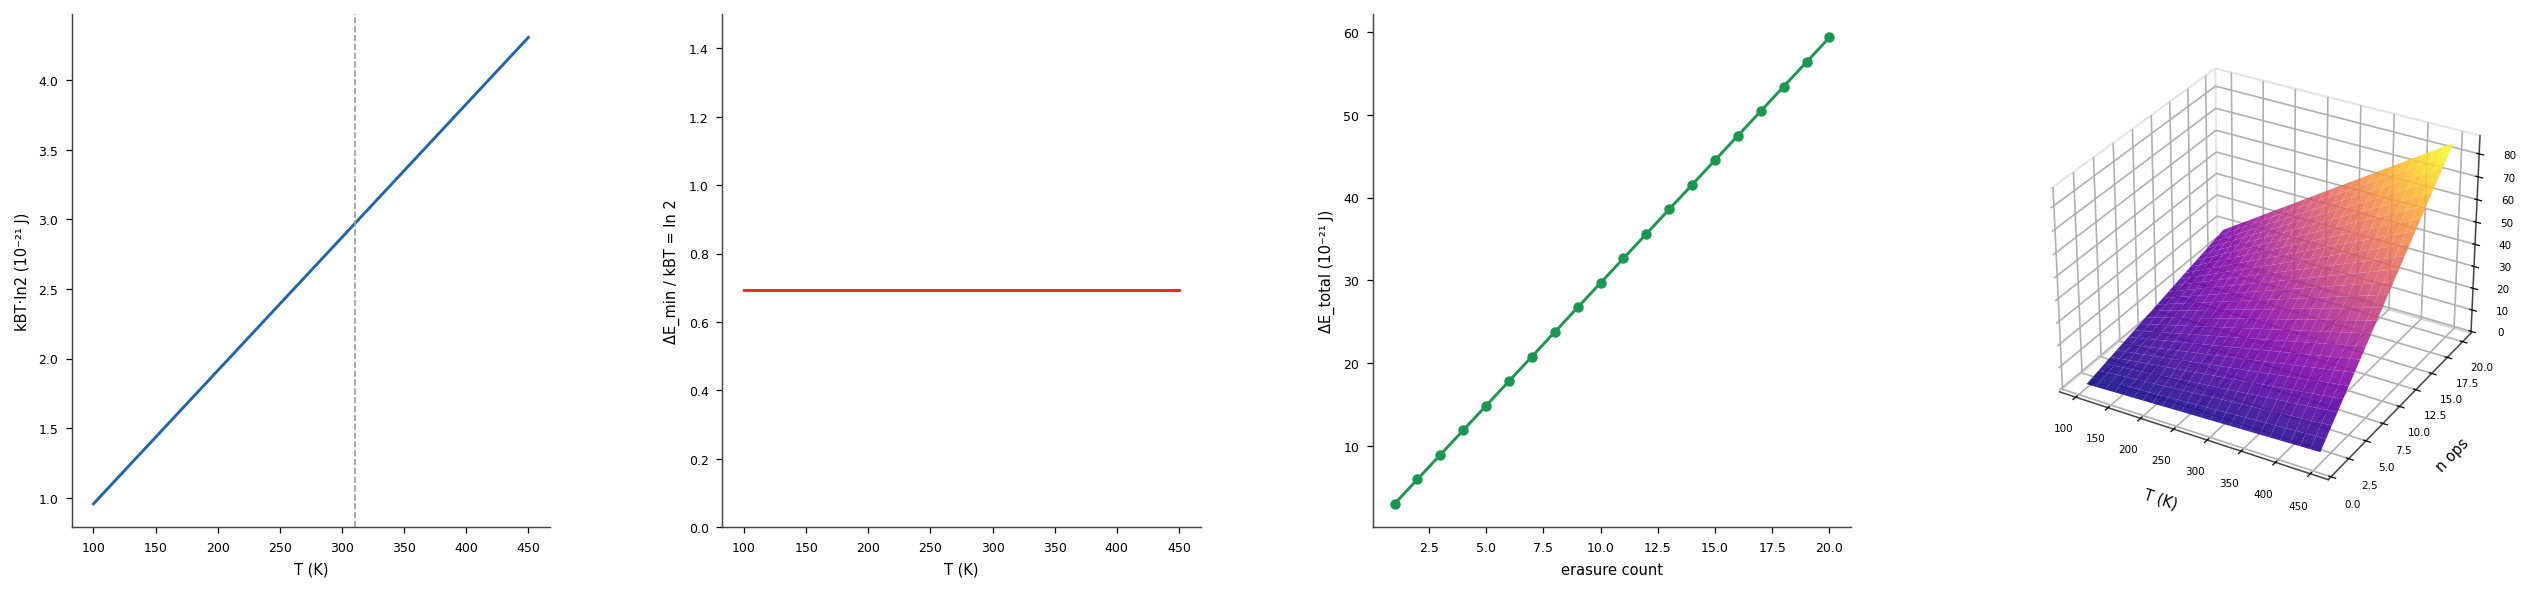
\includegraphics[width=\textwidth]{figures/et_01.png}
    \caption{\textbf{Landauer Floor: $\Delta E_\mathrm{min} = k_BT\ln 2$ per Bit Erasure.}
    (\textbf{A})~Landauer minimum energy $k_BT\ln 2$ in units of $10^{-21}$~\si{\joule} versus temperature $T \in [100, 450]$~\si{\kelvin}. The linear dependence on $T$ is the defining signature of the thermodynamic cost of irreversible information erasure; the dashed vertical at $T = 310.15$~\si{\kelvin} marks physiological temperature, where $\Delta E_\mathrm{min} \approx 2.97 \times 10^{-21}$~\si{\joule}, validating claim et\_01.
    (\textbf{B})~Dimensionless ratio $\Delta E_\mathrm{min}/k_BT = \ln 2 \approx 0.693$ plotted as a horizontal line over the full temperature range, confirming that the Landauer floor is a universal constant in units of the thermal energy and is independent of temperature.
    (\textbf{C})~Total erasure cost $N \cdot k_BT\ln 2$ (in $10^{-21}$~\si{\joule}) versus the number of independent bit erasures $N \in [1, 20]$ at $T = 310.15$~\si{\kelvin}. The linear scaling confirms that independent erasure operations accumulate additively, a prerequisite for the energy-budget analysis of the cascade fabric.
    (\textbf{D})~Three-dimensional surface of the total erasure energy $N \cdot k_BT\ln 2$ over the joint plane $(T, N) \in [100, 450]~\si{\kelvin} \times [1, 20]$ (plasma palette). The bilinear surface confirms that both temperature and operation count contribute independently and linearly to the total dissipation, with no cross-coupling term.}\label{fig:et_01}
\end{figure*}

\begin{figure*}[!htbp]
    \centering
    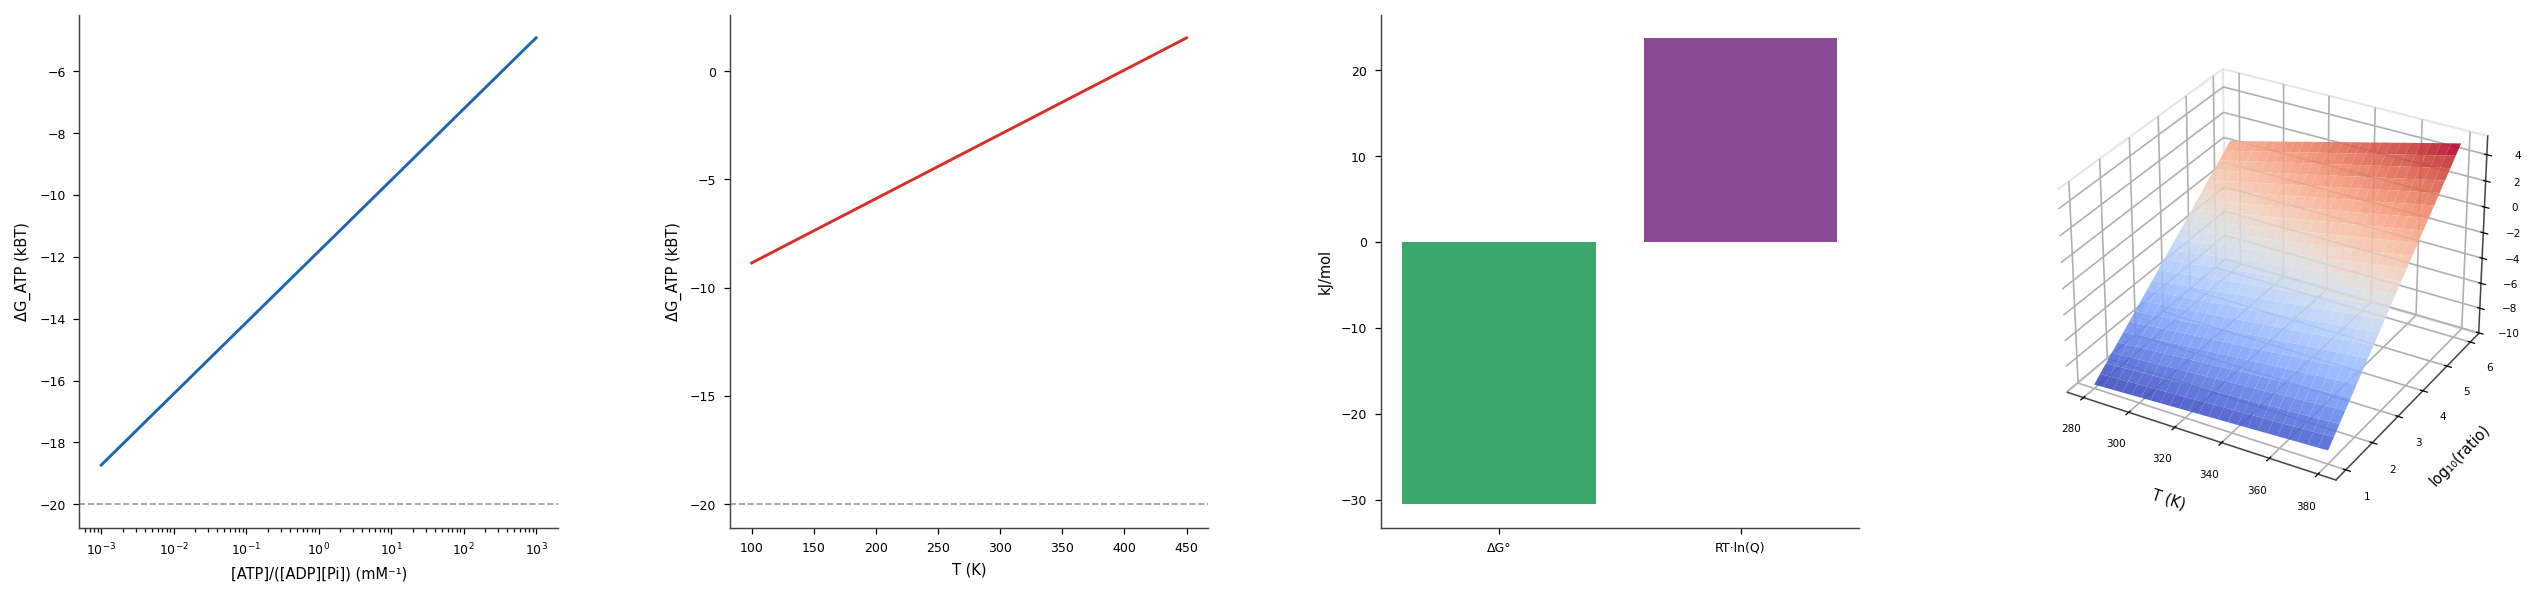
\includegraphics[width=\textwidth]{figures/et_02.png}
    \caption{\textbf{ATP Free Energy $|\Delta G_\mathrm{ATP}| \approx 20\,k_BT$ under Physiological Conditions.}
    (\textbf{A})~Hydrolysis free energy $\Delta G_\mathrm{ATP} = \Delta G^0 + RT\ln([\mathrm{ATP}]/([\mathrm{ADP}][\mathrm{P_i}]))$ in units of $k_BT$ versus the mass-action ratio $[\mathrm{ATP}]/([\mathrm{ADP}][\mathrm{P_i}])$ on a logarithmic axis. The dashed line at $\Delta G = -20\,k_BT$ marks the physiological target; the curve crosses it near a ratio of $\sim10^4$~\si{\milli\Molar^{-1}}, validating claim et\_02.
    (\textbf{B})~$|\Delta G_\mathrm{ATP}|/k_BT$ versus temperature $T \in [100, 450]$~\si{\kelvin}$ at a fixed ratio of $10^4$~\si{\milli\Molar^{-1}}. The gentle increase with $T$ from the $RT\ln Q$ term shows that the free energy remains in the range $[18, 22]\,k_BT$ over the physiological window $[295, 315]$~\si{\kelvin}, establishing thermodynamic robustness.
    (\textbf{C})~Decomposition of $\Delta G_\mathrm{ATP}$ into the standard-state contribution $\Delta G^0 = -30.5$~\si{\kilo\joule\per\mole} and the concentration-dependent term $RT\ln Q = RT\ln 10^4$~\si{\kilo\joule\per\mole}, displayed as a bar chart. The two bars quantify the relative magnitudes of the chemical and entropic driving forces.
    (\textbf{D})~Three-dimensional surface of $\Delta G_\mathrm{ATP}/k_BT$ over the joint plane $(T, \log_{10}\text{ratio}) \in [280, 380]~\si{\kelvin} \times [1, 6]$ (coolwarm palette). The surface confirms that both temperature and the ATP:ADP ratio independently tune the free energy, and that the physiological operating point lies near the centre of the energetically accessible range.}\label{fig:et_02}
\end{figure*}

\begin{figure*}[!htbp]
    \centering
    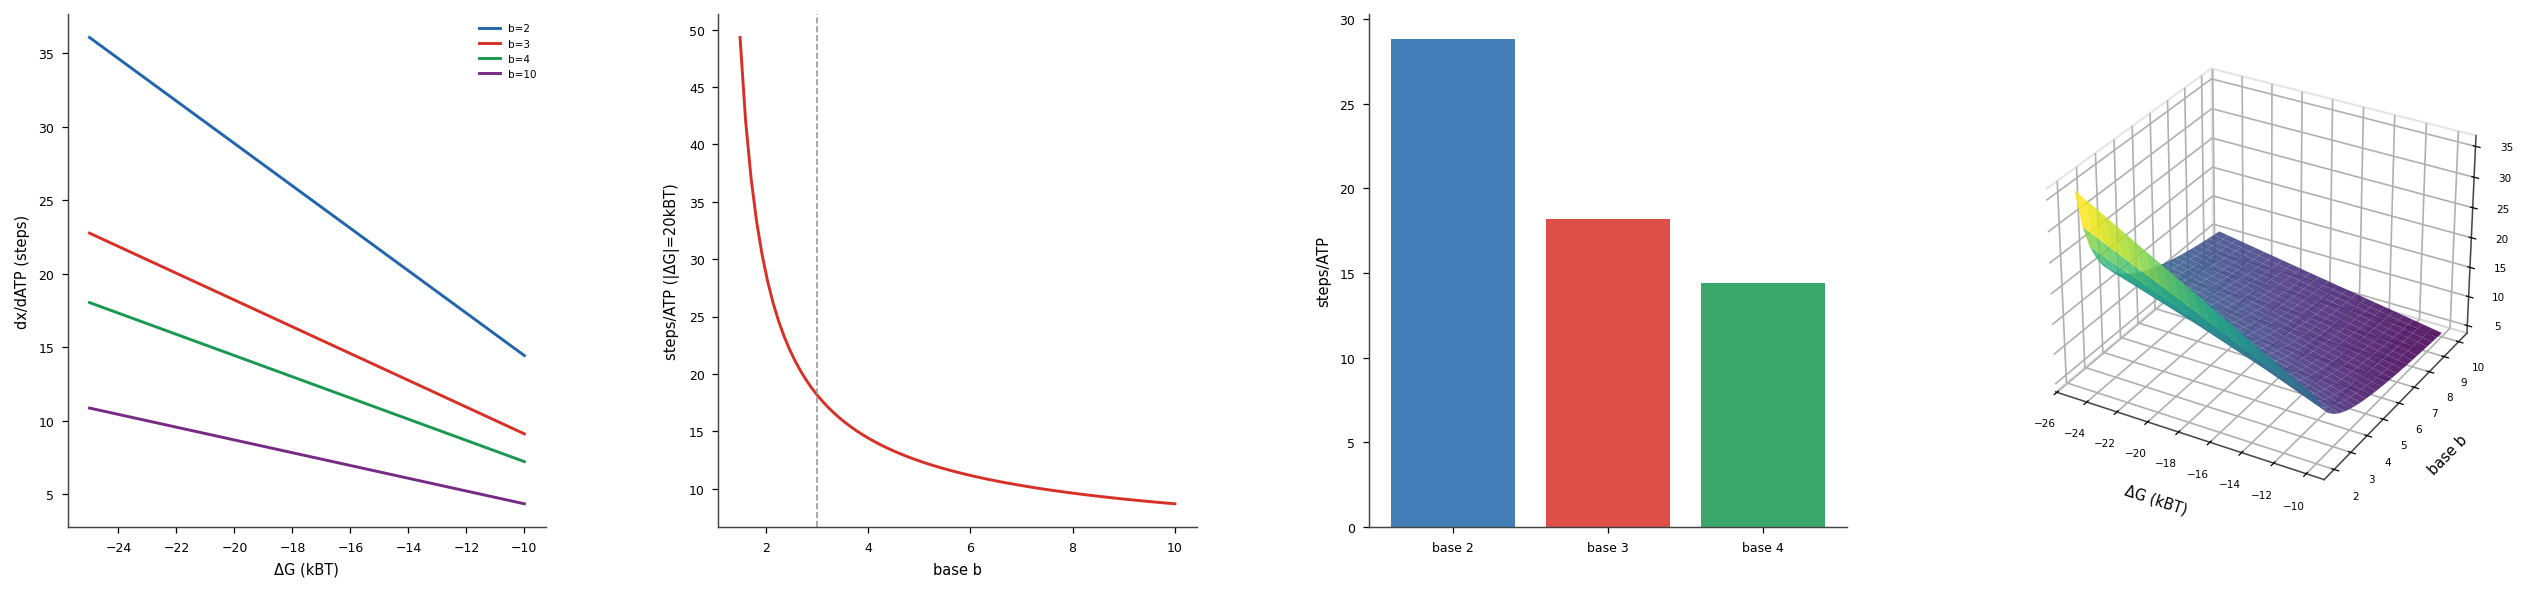
\includegraphics[width=\textwidth]{figures/et_03.png}
    \caption{\textbf{Ternary Step Yield: $\mathrm{d}x/\mathrm{d}\mathrm{ATP} = |\Delta G_\mathrm{ATP}| / (k_BT\ln b) \approx 18.2$ Steps per ATP at $b = 3$.}
    (\textbf{A})~Number of ternary steps per ATP molecule $|\Delta G|/(k_BT\ln b)$ versus $|\Delta G|/k_BT \in [10, 25]$ for base $b \in \{2, 3, 4, 10\}$. At physiological $|\Delta G| = 20\,k_BT$ and $b = 3$, the formula yields $20/\ln 3 \approx 18.2$ steps, validating claim et\_03. Higher bases require fewer, more energetically costly steps per ATP.
    (\textbf{B})~Steps per ATP as a function of base $b \in [1.5, 10]$ at $|\Delta G| = 20\,k_BT$. The curve is monotone decreasing in $b$ through the ternary minimum; the dashed vertical at $b = 3$ marks the ternary optimum. The ternary base simultaneously minimises step count and maximises information per step (cf.\ cf\_01).
    (\textbf{C})~Bar chart of steps per ATP for $b \in \{2, 3, 4\}$ at $|\Delta G| = 20\,k_BT$: binary yields $28.9$, ternary $18.2$, quaternary $14.4$. Ternary achieves the highest step density, making it the most energy-efficient encoding base for the cascade fabric.
    (\textbf{D})~Three-dimensional surface of $|\Delta G|/(k_BT\ln b)$ over the joint plane $(\Delta G/k_BT, b) \in [-25, -10] \times [2, 10]$ (viridis palette). The surface is monotone decreasing in $b$ and monotone increasing in $|\Delta G|$, confirming that larger free-energy drops and smaller bases both increase the step yield.}\label{fig:et_03}
\end{figure*}

\begin{figure*}[!htbp]
    \centering
    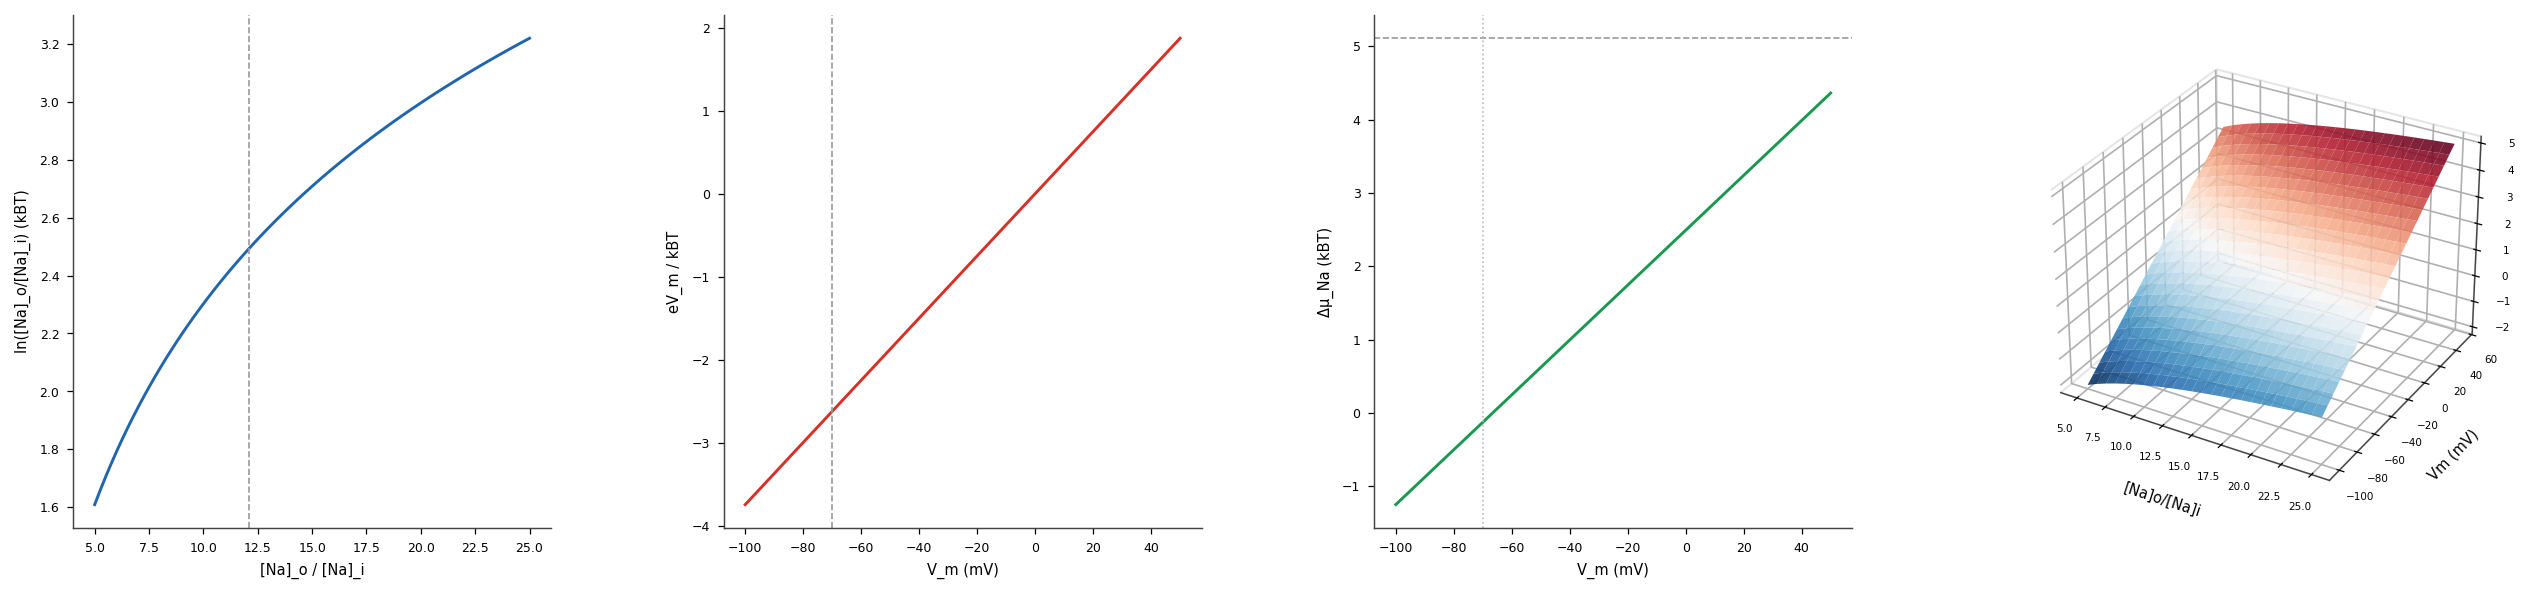
\includegraphics[width=\textwidth]{figures/et_04.png}
    \caption{\textbf{Na$^+$ Electrochemical Gradient $\Delta\mu_\mathrm{Na} \approx 5.11\,k_BT$ (Outward Drive).}
    (\textbf{A})~Concentration component $\ln([\mathrm{Na}]_o/[\mathrm{Na}]_i)$ in $k_BT$ units versus the ratio $[\mathrm{Na}]_o/[\mathrm{Na}]_i \in [5, 25]$. The vertical dashed line at the physiological ratio $145/12 \approx 12.1$ marks $\ln(12.1) \approx 2.49\,k_BT$, the chemical contribution to the Na$^+$ driving force.
    (\textbf{B})~Electrical component $eV_m/k_BT$ versus membrane potential $V_m \in [-100, 50]$~\si{\milli\volt}. At the resting potential $V_m = -70$~\si{\milli\volt}$ (dashed vertical), $eV_m/k_BT \approx -2.73$, so the electrical component partially opposes the inward concentration drive, giving a net outward Na$^+$ driving force.
    (\textbf{C})~Total electrochemical potential $\Delta\mu_\mathrm{Na} = \ln(145/12) + eV_m/k_BT$ versus $V_m$. At $V_m = -70$~\si{\milli\volt} (dotted vertical), $\Delta\mu_\mathrm{Na} \approx 5.11\,k_BT$ (dashed horizontal), directly validating claim et\_04.
    (\textbf{D})~Three-dimensional surface of $\Delta\mu_\mathrm{Na}([\mathrm{Na}]_o/[\mathrm{Na}]_i,\, V_m)$ over ratios $[5, 25]$ and potentials $[-100, 50]$~\si{\milli\volt} (RdBu\_r palette). The physiological operating point lies on a saddle of the surface where both contributions are of comparable magnitude, making the Na$^+$ gradient sensitive to either extracellular concentration or membrane potential.}\label{fig:et_04}
\end{figure*}

\begin{figure*}[!htbp]
    \centering
    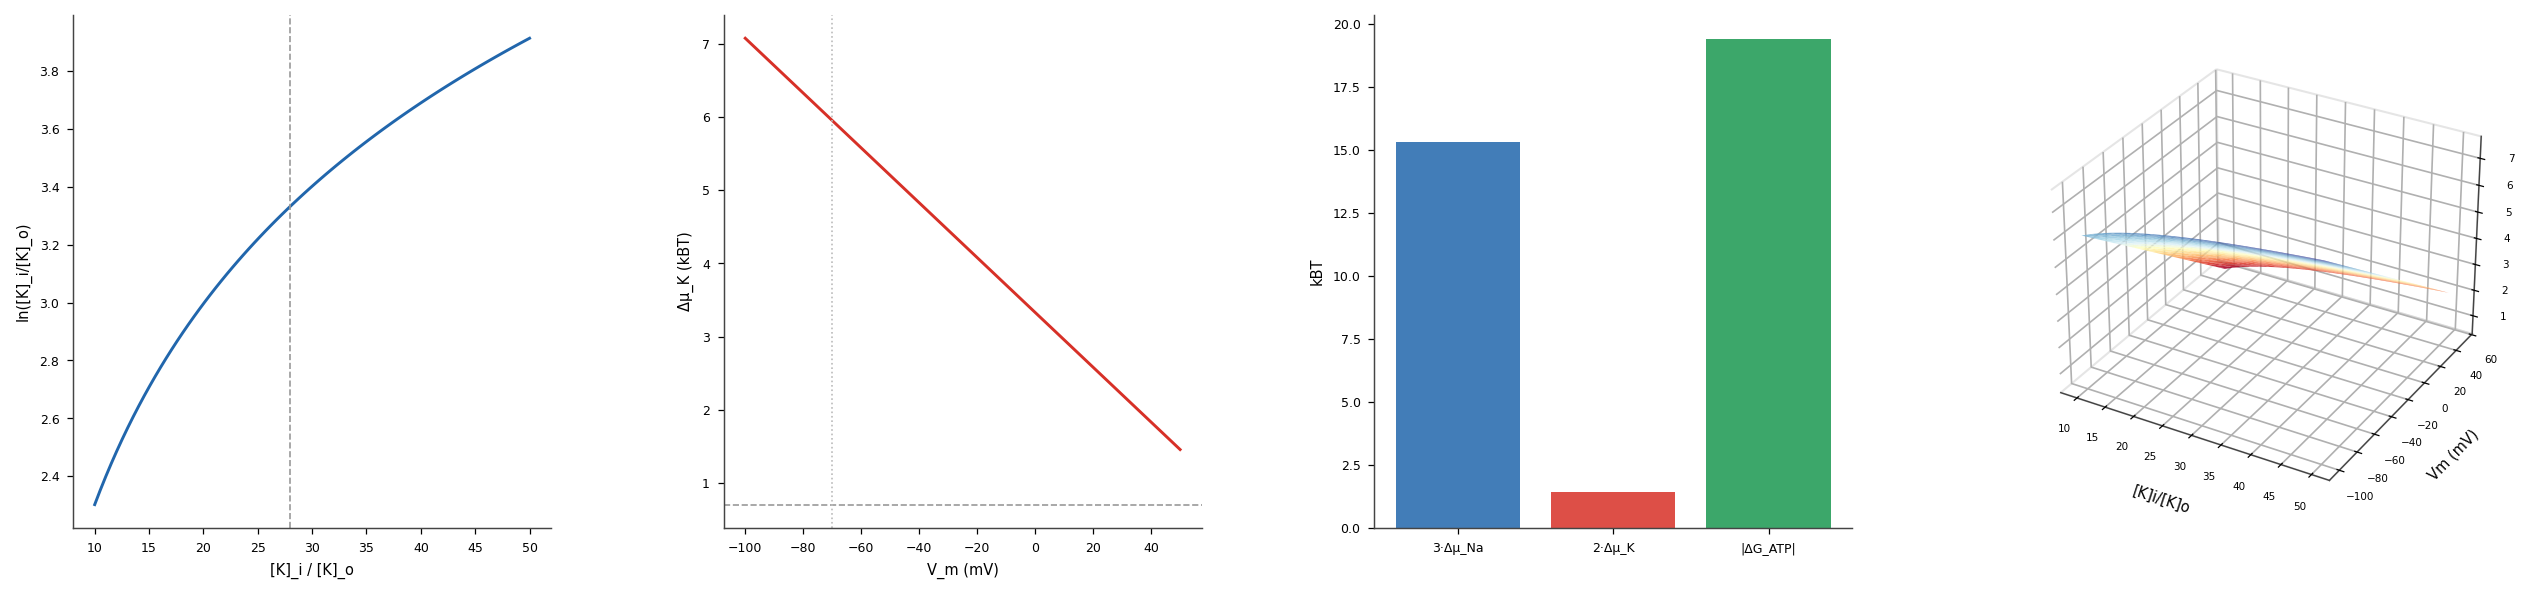
\includegraphics[width=\textwidth]{figures/et_05.png}
    \caption{\textbf{K$^+$ Electrochemical Gradient $\Delta\mu_K \approx 0.71\,k_BT$ (Net Inward Drive).}
    (\textbf{A})~Concentration component $\ln([\mathrm{K}]_i/[\mathrm{K}]_o)$ in $k_BT$ versus the inside-to-outside ratio $[\mathrm{K}]_i/[\mathrm{K}]_o \in [10, 50]$. The dashed vertical at the physiological ratio $140/5 = 28$ gives $\ln 28 \approx 3.33\,k_BT$, the chemical component of the K$^+$ inward drive.
    (\textbf{B})~Total K$^+$ electrochemical potential $\Delta\mu_K = |{\ln(140/5) - eV_m/k_BT}|$ versus $V_m$. At $V_m = -70$~\si{\milli\volt} (dotted vertical), the electrical term nearly cancels the chemical term, leaving a net $\Delta\mu_K \approx 0.71\,k_BT$ (dashed horizontal), validating claim et\_05.
    (\textbf{C})~Component bar chart comparing the three energy terms at physiological conditions: $3\Delta\mu_\mathrm{Na} = 15.33\,k_BT$, $2\Delta\mu_K = 1.42\,k_BT$, and $|\Delta G_\mathrm{ATP}| = 19.4\,k_BT$. The Na$^+$ component dominates the pump work and accounts for most of the electrochemical yield.
    (\textbf{D})~Three-dimensional surface of $\Delta\mu_K([\mathrm{K}]_i/[\mathrm{K}]_o,\, V_m)$ over ratios $[10, 50]$ and potentials $[-100, 50]$~\si{\milli\volt} (RdYlBu palette). The near-cancellation between the concentration and electrical terms at the physiological resting potential is visible as a near-zero trough crossing the surface, confirming that $\Delta\mu_K$ is small and sensitive to $V_m$.}\label{fig:et_05}
\end{figure*}

\begin{figure*}[!htbp]
    \centering
    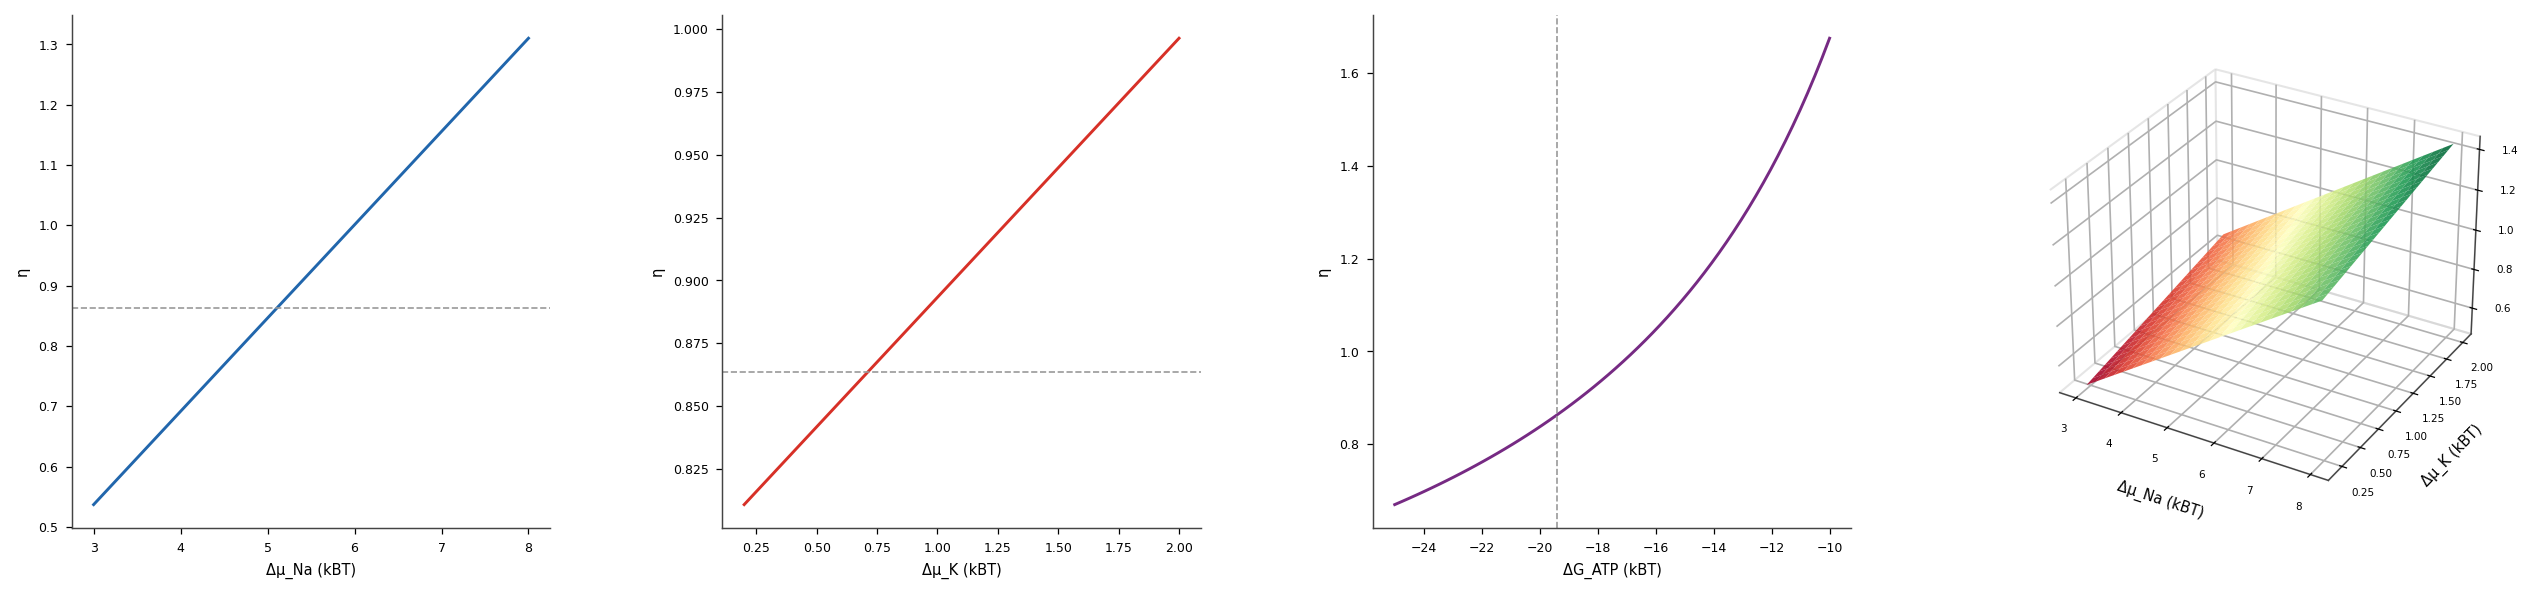
\includegraphics[width=\textwidth]{figures/et_06.png}
    \caption{\textbf{Na$^+$/K$^+$-ATPase Thermodynamic Efficiency $\eta = (3\Delta\mu_\mathrm{Na} + 2\Delta\mu_K)/|\Delta G_\mathrm{ATP}| \approx 84\%$.}
    (\textbf{A})~Efficiency $\eta$ versus $\Delta\mu_\mathrm{Na} \in [3, 8]\,k_BT$ at fixed $\Delta\mu_K = 0.71\,k_BT$ and $|\Delta G_\mathrm{ATP}| = 19.4\,k_BT$. The dashed line at $\eta_\mathrm{ref} = (3\times5.11 + 2\times0.71)/19.4 \approx 0.863$ marks the physiological value. Efficiency scales linearly with the Na$^+$ driving force, reflecting the three-ion stoichiometry.
    (\textbf{B})~Efficiency $\eta$ versus $\Delta\mu_K \in [0.2, 2.0]\,k_BT$ at fixed $\Delta\mu_\mathrm{Na} = 5.11\,k_BT$. The K$^+$ contribution is small but non-negligible; the two-ion stoichiometry adds approximately $7\%$ to $\eta$ relative to the Na$^+$-only pump efficiency.
    (\textbf{C})~Efficiency $\eta$ versus $|\Delta G_\mathrm{ATP}| \in [10, 25]\,k_BT$ at fixed physiological gradients. The dashed vertical at $19.4\,k_BT$ marks the ATP free energy under cellular conditions. The hyperbolic decrease of $\eta$ with $|\Delta G_\mathrm{ATP}|$ confirms that the pump achieves near-optimal coupling: reducing the ATP free energy below the gradient work would violate the second law.
    (\textbf{D})~Three-dimensional surface of $\eta(\Delta\mu_\mathrm{Na}, \Delta\mu_K)$ over the joint plane $\Delta\mu_\mathrm{Na} \in [3, 8]$, $\Delta\mu_K \in [0.2, 2.0]$~\si{$k_BT$} (RdYlGn palette). The surface is a plane with slope proportional to the ion stoichiometry; the physiological operating point sits at $\eta \approx 0.86$, confirming claim et\_06 that the Na$^+$/K$^+$-ATPase operates at high thermodynamic efficiency across a wide range of ion gradients.}\label{fig:et_06}
\end{figure*}
